\documentclass{article}
\usepackage{mathrsfs}
\usepackage{amsmath}
\usepackage{amsthm}
\usepackage{amssymb}
\usepackage{graphicx}
\usepackage{subfigure}
\usepackage{color}
\DeclareMathOperator*{\argmax}{argmax}
%\include{macros}
%\usepackage{floatflt}
%\usepackage{graphics}
%\usepackage{epsfig}


\theoremstyle{definition}
\newtheorem{theorem}{Theorem}[section]
\newtheorem{lemma}[theorem]{Lemma}
\newtheorem{proposition}[theorem]{Proposition}
\newtheorem{corollary}[theorem]{Corollary}

\theoremstyle{definition}
\newtheorem*{defition}{Definition}
\newtheorem*{example}{Example}

\theoremstyle{remark}
\newtheorem*{remark}{Remark}
\newtheorem*{note}{Note}
\newtheorem*{exercise}{Exercise}

\setlength{\oddsidemargin}{-0.25 in}
\setlength{\evensidemargin}{-0.25 in} \setlength{\topmargin}{-0.25
in} \setlength{\textwidth}{7 in} \setlength{\textheight}{8.5 in}
\setlength{\headsep}{0.25 in} \setlength{\parindent}{0 in}
\setlength{\parskip}{0.1 in}

\newcommand{\homework}[4]{
\pagestyle{myheadings} \thispagestyle{plain}
\newpage
\setcounter{page}{1} \setcounter{section}{#4} \noindent
\begin{center}
\framebox{ \vbox{\vspace{2mm} \hbox to 6.28in { {\bf
THU-70250043,~Pattern~Recognition~(Spring 2016) \hfill Homework: 1} }
\vspace{6mm} \hbox to 6.28in { {\Large \hfill #1 \hfill} }
\vspace{6mm} \hbox to 6.28in { {\it Lecturer: #2 \hfill} }
\vspace{2mm} \hbox to 6.28in { {\it Student: #3 \hfill} }
\vspace{2mm} } }
\end{center}
\markboth{#1}{#1} \vspace*{4mm} }


\begin{document}

\homework{Bayesian Methods}{Changshui Zhang
\hspace{5mm} {\tt zcs@mail.tsinghua.edu.cn}}{Qingfu Wen (2015213495)\hspace{5mm} {\tt qingfu.wen@gmail.com
 } }{8}

%%%%%%%%%%%%%%%%%%%%%%%%%%%%%%%%%%%%%%%%%%%%%%%%%%%%%%%%%%%%%%%%%%%%
% Section 2.  Problem
%%%%%%%%%%%%%%%%%%%%%%%%%%%%%%%%%%%%%%%%%%%%%%%%%%%%%%%%%%%%%%%%%%%%

\section*{Probability}

1. Conditional probability

1.1. Prove that $P(A\cap B \cap C)=P(A|B,C)P(B|C)P(C)$.

\emph{\textbf{PROOF}}:\\
$\because P(A|B,C)= \frac{P(ABC)}{P(BC)}$, $P(B|C)=\frac{P(BC)}{P(C)}$.

$\therefore P(A|B,C)P(B|C)P(C)=\frac{P(ABC)}{P(BC)}*\frac{P(BC)}{P(C)}*P(C)=P(ABC)=P(A\cap B \cap C)$

1.2. Suppose we play a game where I present to you three doors, one of which has a prize behind. The
doors are closed and so you choose a door which you think conceals the prize. After you make your
choice, I open one of the two doors you didn't pick, and reveal that the prize wasn't there (note that
I can always do this). Then I give you the choice whether to stick with your current door, or switch
to the remaining un-opened door. What should you do to have the highest probability of winning the
prize?

\emph{\textbf{SOLUTION}}:\\
Switch the door.\\
$P(stick)=\frac{1}{3}$, $P(switch)=\frac{2}{3}$.

2. Suppose that I have two six-sided dice, one is fair and the other one is loaded, i.e.
$$ P(x)=\left\{
\begin{aligned}
&\frac{1}{3},x=6 \\
&\frac{2}{15},x\in\{1,2,3,4,5\}.
\end{aligned}
\right.
$$
I will toss a coin to decide which die to roll. If the coin flip is heads I will roll the fair die, otherwise the
loaded one. The probability that the coin flip is heads is $p\in(0,1)$.

2.1. What is the expectation of the die roll (in terms of $p$).\\
\emph{\textbf{SOLUTION}}:
\begin{equation}\nonumber
P(y)=\left\{
\begin{array}{lll}
\frac{1}{6}p+\frac{1}{3}(1-p),y=6\\
\frac{1}{6}p+\frac{2}{15}(1-p),y\in\{1,2,3,4,5\}
\end{array} \right.=\left\{
\begin{array}{lll}
\frac{1}{3}-\frac{1}{6}p,y=6\\
\frac{2}{15}+\frac{1}{30}p,y\in\{1,2,3,4,5\}
\end{array} \right.
\end{equation}
$E(Y) = 6*(\frac{1}{3}-\frac{1}{6}p)+15*(\frac{2}{15}+\frac{1}{30}p)=4-\frac{1}{2}p$


2.2. What is the variance of the die roll (in terms of $p$).\\
\emph{\textbf{SOLUTION}}:\\
$E(Y) = 4-\frac{1}{2}p$\\
$Var(Y) = E(Y^2)-[E(Y)]^2 = 36*(\frac{1}{3}-\frac{1}{6}p)+(1+4+9+16+25)(\frac{2}{15}+\frac{1}{30}p)-(4-\frac{1}{2}p)^2
=-\frac{1}{4}p^2-\frac{1}{6}p+\frac{10}{3}$

3. Assume that $A$ and $B$ are two events and $A^c$ is the complement of $A$. Prove the following:

3.1. $P(B\cap A^c)=P(B)-P(A\cap B),$\\
\emph{\textbf{PROOF}}:\\
$\because P(B\cap A^c)+P(B\cap A) = P(B), \therefore P(B\cap A^c)=P(B)-P(A\cap B).$

3.2. $P(A\cup B) = P(A)+P(B)-P(A\cap B),$\\
\emph{\textbf{PROOF}}:\\
$\forall A, B$, we have $P(A-B) = P(A)-P(AB)$.\\
$\because A\cup B = A \cup (B-A)$ and $A\cap(B-A)=\varnothing$. \\
$\therefore P(A\cup B)=P(A)+P(B-A)=P(A)+P(B)-P(AB)$.

3.3. $(A\cap B)^c = A^c\cup B^c$,\\
\emph{\textbf{PROOF}}:\\
$\forall x \in (A\cap B)^c \Rightarrow x \not\in A\cap B \Rightarrow x\in A^c$ or $A\in B^c\Rightarrow A^c\cup B^c$.\\
$\forall x \in A^c\cup B^c \Rightarrow x \in A^c$ or $x \in B^c\Rightarrow x\not\in A$ and $x \not\in B\Rightarrow x \in (A\cap B)^c $.\\
Thus, $(A\cap B)^c = A^c\cup B^c$.

3.4. $P(A\cap B)\geq P(A)+P(B)-1$.\\
\emph{\textbf{PROOF}}:\\
From 3.2, $P(A\cup B) = P(A)+P(B)-P(A\cap B) \leq 1$. Thus, $P(A\cap B)\geq P(A)+P(B)-1$.

4. Random variables.

4.1 Show that the following functions are Cumulative Distribution Function (CDF):\\
$F(x)=\frac 1 2 + \frac 1 \pi \arctan x$, for $x\in(-\infty,\infty)$,\\
$F(x)=(1+e^{-x})^{-1}$, for $x\in(-\infty,\infty)$,\\
$F(x)=e^{-e^{-x}}$, for $x\in(-\infty,\infty)$,\\
$F(x)=1-e^{-x}$, for $x\in[0,\infty)$.

\emph{\textbf{PROOF}}:\\
if $F(x)$ is CDF, $F(x)$ have the following properties.
\begin{itemize}
\item $\lim\limits_{x \to -\infty }{F(x)} = 0, \lim\limits_{x \to +\infty }{F(x)} = 1$
\item if $x_1<x_2$, $F(x_1)\leq F(x_2)$
\item $\lim\limits_{x \to x_0^+}{F(x)} = 0$
\end{itemize}

\begin{enumerate}
\item[1)] $F(x)=\frac 1 2 + \frac 1 \pi \arctan x, x\in(-\infty,\infty)$, It is a non-decreasing function and right continuous.\\
$\lim\limits_{x \to -\infty }{F(x)} =\frac{1}{2}+\frac{1}{\pi}*(-\frac{\pi}{2})= 0, \lim\limits_{x \to +\infty }{F(x)} =\frac{1}{2}+\frac{1}{\pi}*(\frac{\pi}{2})= 1$
\item[2)] $F(x)=(1+e^{-x})^{-1}$, for $x\in(-\infty,\infty)$, It is a non-decreasing function and right continuous.\\
$\lim\limits_{x \to -\infty }{F(x)} =(1+\infty)^(-1)= 0, \lim\limits_{x \to +\infty }{F(x)} =(1+0)^(-1)= 1$
\item[3)] $F(x)=e^{-e^{-x}}$, for $x\in(-\infty,\infty)$, It is a non-decreasing function and right continuous.\\
$\lim\limits_{x \to -\infty }{F(x)} =e^{-\infty}= 0, \lim\limits_{x \to +\infty }{F(x)} =e^{0}= 1$
\item[4)] $F(x)=1-e^{-x}$, for $x\in[0,\infty)$, It is a non-decreasing function and right continuous.\\
$\lim\limits_{x \to 0^+ }{F(x)} =1-1= 0, \lim\limits_{x \to +\infty }{F(x)} =1-e^{-\infty}= 1$
\end{enumerate}

4.2. Consider variables $X\sim F_X$ and $Y\sim F_Y$, where $F_X$ and $F_Y$ are CDFs. Assume that $F_X$ is stochastically greater than $F_Y$, that is for all $t$,
$F_X(t) \leq F_Y(t)$ and moreover there exists some $t$ with $F_X(t) < F_Y(t)$. Show that $X$ tends to be bigger than $Y$, that is
for all $t$ we have $P(X>t)\geq P(Y>t)$ and there exists some $t$ such that $P(X>t)> P(Y>t)$.\\
\emph{\textbf{PROOF}}:\\
$\because \forall t$, $F_X(t) \leq F_Y(t)$ and exists some $t$ with $F_X(t) < F_Y(t)$.\\
$\therefore \forall t, 1- F_X(t) \geq 1-F_Y(t)$ and exists some $t$ with $1-F_X(t) > 1-F_Y(t)$.\\
$\therefore \forall t, P(X>t) \geq P(Y>t)$ and exists some $t$ with $P(X>t) > P(Y>t)$.\\


5. Conditional independence.

The notation $X\perp Y$ indicates that random variables $X$ and $Y$ are independent. Similarly, $X\perp Y|Z$ means that $X$ and $Y$ are conditionally independent given $Z$,
that is $p(x,y|z)=p(x|z)p(y|z)$.

Prove or disprove via a counter example the following statements about conditional independence:\\
$(X\perp (Y,W)|Z)$ implies $(X\perp Y|Z)$,\\
$(X\perp Y|Z)$ and $(X,Y\perp W|Z)$ implies $(X\perp W|Z)$,\\
$(X\perp (Y,W)|Z)$ and $(Y\perp W|Z)$ implies $(X,W\perp Y|Z)$.\\
\emph{\textbf{PROOF}}:
\begin{enumerate}
\item[1)] $\because P(X,Y|Z)=\sum_{w}P(X, Y, w|Z)=\sum_{w}P(X|Z)P(Y,w|Z)=P(X|Z)P(Y|Z)$\\
    $\therefore(X\perp (Y,W)|Z) \Rightarrow (X\perp Y|Z)$.
\item[2)] $\because P(X,W|Z)=\sum_{y}P(X, Y, y|Z)=\sum_{y}P(X,y|Z)P(W|Z)=\sum_{y}P(X|Z)P(y|Z)P(W|Z)=P(X|Z)P(W|Z)$\\
    $\therefore(X\perp Y|Z)$ and $(X,Y\perp W|Z) \Rightarrow (X\perp W|Z)$.
\item[3)] $\because P(X,W|Z)=\sum_{y}P(X,y,W|Z)=\sum_{y}P(X|Z)P(y,W|Z)=P(X|Z)P(W|Z)$\\
    $P(X,W,Y|Z)=P(X|Z)P(Y,W|Z)=P(X|Z)P(Y|Z)P(W|Z)=P(X,W|Z)P(Y|Z)$\\
    $\therefore(X\perp (Y,W)|Z)$ and $(Y\perp W|Z) \Rightarrow (X,W\perp Y|Z)$.
\end{enumerate}

\section*{Gaussian in High Dimensions}

A great deal of current work in machine learning is concerned with data which are in a high dimensional
space (for example text documents, which may be seen as vectors in the lattice points of $\mathbb{R}^d$
where d is the number of words in the language). In this problem we will see that we must be careful when porting familiar
concepts from the loving embrace of $\mathbb{R}^3$ into higher dimensions.

Consider the d..dimensional Gaussian distribution:
\[
x\sim ~N(0^{d\times 1}, I^{d\times d})
\]
where $I^{d\times d}$ is the identity matrix of size $d\times d$.

1. Show that the distribution of $\lVert x \rVert_2^2$ is the same say the distribution of $T_d=\sum_{i=1}^d y_i^2$ where $y_t\sim ~N(0,1)$ are independent.\\
\emph{\textbf{PROOF}}:\\
$\because x\sim ~N(0^{d\times 1}, I^{d\times d})$\\
$\therefore \forall i\neq j, x_i,x_j$are independent and $x_i\sim ~N(0,1).$\\
$\therefore \lVert x \rVert_2^2 = \sum_{i=1}^d x_i^2$ is the same distribution of $T_d$.

2. Compute the mean and variance of $y_i^2$.\\
\emph{\textbf{SOLUTION}}:\\
$E(y_i^2) = Var(y_i)+E(y_i)^2 = 1 + 0 = 1$.\\
$Var(y_i^2) = E(y_i^4)-E(y_i^2)^2 = \frac{1}{\sqrt{2\pi}}\int_{-\infty}^{+\infty}y_i^4 e^{-\frac{y_i^2}{2}}\,dy - 1 =  3 - 1 = 2.$

3. Compute the mean and variance of $T_d$.\\
\emph{\textbf{SOLUTION}}:\\
$E(T_d)=E(\sum_{i=1}^d y_i^2) = \sum_{i=1}^d E(y_i^2)=d$ \\
$Var(T_d)=Var(\sum_{i=1}^d y_i^2)=2d$

4. Show that $P(d-10\sqrt{2d}\leq T_d \leq d+10\sqrt{2d})\geq 0.99$, for suitably large $d$. Tip: you may use the Chebyshev's Inequality.\\
\emph{\textbf{PROOF}}:\\
From Chebyshev's Inequality, we have
\[ P(|T_d-d|\geq10\sqrt{2d})\leq\frac{1}{10^2}\]
$\therefore P(T_d \leq d-10\sqrt{2d})+P(T_d \geq d+10\sqrt{2d})\leq0.01$\\
$\therefore P(d-10\sqrt{2d}\leq T_d \leq d+10\sqrt{2d})\geq 0.99$.

5. Prove that your answer above implies that $P(\sqrt d - 20 \leq \sqrt{T_d} \leq \sqrt d + 20)\geq 0.99$.\\
\emph{\textbf{PROOF}}:\\
$P(\sqrt d - 20 \leq \sqrt{T_d} \leq \sqrt d + 20) = P(d - 40\sqrt d+400\leq \sqrt{T_d} \leq  d + 40\sqrt d +400) $\\
when $d$ is large enough, $d - 40\sqrt d+400\leq d-10\sqrt{2d}$ and $d + 40\sqrt d +400\geq d+10\sqrt{2d}$.\\
$\therefore P(\sqrt d - 20 \leq \sqrt{T_d} \leq \sqrt d + 20) = P(d - 40\sqrt d+400\leq \sqrt{T_d} \leq  d + 40\sqrt d +400) \geq P(d-10\sqrt{2d}\leq T_d \leq d+10\sqrt{2d})\geq 0.99.$
\section*{Bernstein's inequality}

Recall Bernstein's inequality. Let $X_1,...,X_2$ be iid with mean $\mu$ and variance $\sigma^2$ and suppose that $|X_t|\leq c$. Then
\[
P(|\bar{X}_n-\mu|>\epsilon)\leq 2\exp\left(-\frac{n\epsilon^2}{2\sigma^2+\frac{2c\epsilon}{3}}\right)
\]
where $\bar{X}_n=n^{-1}\sum_{i=1}^n X_i$.

1. Shaw that, with probability at least $1-2\delta$,
\[
|\bar{X}_n-\mu| \leq \sqrt{\frac{2\sigma^2\log(1/\delta)}{n}}+\frac{2c\log(1/\delta)}{3n}.
\]
\emph{\textbf{PROOF}}:\\
\begin{equation}\nonumber
\begin{aligned}
P\left(|\bar{X}_n-\mu| \leq \sqrt{\frac{2\sigma^2\log(1/\delta)}{n}}+\frac{2c\log(1/\delta)}{3n}\right)&=1-P\left(|\bar{X}_n-\mu| >\sqrt{\frac{2\sigma^2\log(1/\delta)}{n}}+\frac{2c\log(1/\delta)}{3n}\right)\\
             &\geq 1- 2\exp\left(-\frac{n(\sqrt{\frac{2\sigma^2\log(1/\delta)}{n}}+\frac{2c\log(1/\delta)}{3n})^2}{2\sigma^2
             +\frac{2c(\sqrt{\frac{2\sigma^2\log(1/\delta)}{n}}+\frac{2c\log(1/\delta)}{3n})}{3}}\right)\\
            &\geq 1-2\exp\left(-\log(1/\delta)\right)\\
            &=1-2\delta
\end{aligned}
\end{equation}

2. Let $Y_1,...,Y_n$ be iid random variables with bounded density $f$. Let $A_n=[-1/n,1/n]$. Define $X_i=I(Y_i\in A_n)$. Let $\mu_n=\mathbb{E}(X_i)=P(Y_i\in A_n)$.
Use Bernstein's inequality to show that for any $\delta > 0$,
\[
P\left(|\bar{X}_n-\mu_n|\geq \frac{C}{n}\right)\leq \delta,
\]
where constant $C$ is irrelevant of $n$.\\
\emph{\textbf{PROOF}}:\\
First of all, $|X_i|\leq1$, $\mu_n=\mathbb{E}(X_i)=P(Y_i\in A_n)$, $\delta^2\leq\mu_n(1-\mu_n)\leq\mu_n$. Suppose$M = \sup f$, then $\delta^2\leq\mu_n\leq\frac{M}{n}$.
from Bernstein's inequality, we set $\epsilon=\frac{C}{n}$. Then we get
\begin{equation}\nonumber
\begin{aligned}
P\left(|\bar{X}_n-\mu_n|\ge\frac{C}{n}\right)&\leq2\exp\left(-\frac{n*(\frac{C}{n})^2}{2\sigma^2+\frac{2cC}{3n}}\right)\\
            &\leq2\exp\left(-\frac{\frac{C^2}{n}}{\frac{2M}{n}+\frac{2cC}{3n}}\right)\\
            &=2\exp\left(-\frac{C^2}{2M+\frac{2cC}{3}}\right)
\end{aligned}
\end{equation}
When $C\rightarrow\infty, 2\exp\left(-\frac{C^2}{2M+\frac{2cC}{3}}\right)\rightarrow 0$. Thus, for any $\delta > 0$,
\[
P\left(|\bar{X}_n-\mu_n|\geq \frac{C}{n}\right)\leq \delta,
\]
\section*{MLE and MAP}

Maximum Likelihood Estimation (MLE) and Maximum A Posterior (MAP) are two basic principles for
learning parametric distributions. In this problem you will derive the MLE and the MAP estimates for some
widely-used distributions.

Before stating the problems, we first give a brief review of MLE and MAP. Suppose we consider a family of
distributions (c.d.f or p.m.f.) $F:=\{f(x|\theta):\theta\in\Theta\}$, where x denotes the random vector, $\theta$
denotes a vector of parameters, and $\Theta$ denotes the set of all possible values of $\theta$. Given a set
$\{x_1,x_2,...,x_n\}$ of sample points independently drawn from some $f^*\in F$, or equivalently some $f(x|\theta^*)$
such that $\theta^*\in \Theta$, we want to obtain an estimate of the value of $\theta^*$. Recall that in the case
of an independently and identically distributed(i.i.d.) sample the log-likelihood function is in the following
form
\[
l(\theta)=\sum_{i=1}^n \log f(x_i|\theta),
\]
which is a function of $\theta$ under some fixed sample $\{x_1,x_2,...,x_n\}$. The MLE estimate $\hat{\theta}_{mle}$ is
then defined as follows:
\begin{itemize}
  \item $\hat{\theta}_{mle}\in\Theta$,
  \item $\forall \theta\in\Theta,$ $l(\theta)\leq l(\hat{\theta}_{mle})$.
\end{itemize}

If we have access to some prior distribution $P(\theta)$ over $\Theta$, be it from past experiences or domain knowledge
or simply belief, we can think about the posterior distribution over $\Theta$:
\[
q(\theta):=\frac{\left(\prod_{i=1}^nf(x_t|\theta)\right)p(\theta)}{z(x_1,x_2,...,x_n)},
\]
where
\[
z(x_1,x_2,...,x_n):=\int_\Theta \left(\prod_{i=1}^nf(x_t|\theta)\right)p(\theta) d\theta.
\]
The MAP estimate $\hat{\theta}_{map}$ is then defined as follows:
\begin{itemize}
  \item $\hat{\theta}_{map}\in \Theta$,
  \item $\forall \theta \in \Theta,$ $q(\theta)\leq q(\hat{\theta}_{map})$, or equivalently,
  \[
  l(\theta)+\log p(\theta) \leq l(\hat{\theta}_{map}) + \log p(\hat{\theta}_{map}).
  \]
\end{itemize}

1. The Poisson distribution is useful for modeling the number of events occurring within a unit time, such
as the number of packets arrived at some server per minute. The probability mass function of a Poisson
distribution is as follows:
\[
P(k|\lambda):= \frac{\lambda^k e^{-\lambda}}{k!},
\]
where $\lambda > 0$ is the parameter of the distribution and $k\in\{0,1,2,...\}$ is the discrete random variable modeling
the number of events encountered per unit time.

1.1. Let $\{k_1,k_2,...,k_n\}$ be an i.i.d. sample drawn from a Poisson distribution with parameter $\lambda$. Derive the MLE estimate $\hat{\lambda}_{mle}$
of $\lambda$ based on this sample.\\
\emph{\textbf{SOLUTION}}:\\
\begin{equation}\nonumber
\begin{aligned}
l(\lambda)&=\prod\limits_{i=1}^{n}\frac{\lambda^{k_i} e^{-n\lambda}}{k_i!}=\frac{\lambda^{\sum\limits_{i=1}^n k_i} e^{-\lambda}}{\prod\limits_{i=1}^{n}k_i!}\\
\frac{\partial l(\lambda)}{\partial \lambda}&=\frac{\sum\limits_{i=1}^n k_i\lambda^{\sum k_i - 1} e^{-n\lambda}-n\lambda^{\sum k_i} e^{-n\lambda}}{\prod\limits_{i=1}^{n}k_i!}=0
\end{aligned}
\end{equation}
we get $\hat{\lambda}_{mle} = \frac{\sum\limits_{i=1}^n k_i}{n}$.

1.2. Let K be a random variable following a Poisson distribution with parameter $\lambda$. Derive its mean E[K] and variance Var[K]. Since $\hat{\lambda}_{mle}$
depends on the sample used for estimation, it is also a random variable. Derive the mean and the variance of $\hat{\lambda}_{mle}$, and compare them with E[K]
and Var[K]. What do you find?\\
\emph{\textbf{SOLUTION}}:\\
$E[K]=\sum\limits_{k=0}^{+\infty}k\frac{\lambda^k e^{-\lambda}}{k!}=\sum\limits_{k=1}^{+\infty}\frac{\lambda^{k-1}\lambda e^{-\lambda}}{(k-1)!}=\lambda e^{-\lambda}\sum\limits_{k=0}^{+\infty}\frac{\lambda^{k}}{k!}=\lambda e^{-\lambda}e^{\lambda}=\lambda$.\\
$Var[K]=E[K^2]-E^2[K]=\sum\limits_{k=0}^{+\infty}k^2\frac{\lambda^k e^{-\lambda}}{k!}-\lambda^2=\lambda e^{-\lambda}(\sum\limits_{k=1}^{+\infty}\lambda\frac{\lambda^{k-2}}{(k-2)!}+\sum\limits_{k=1}^{+\infty}
\frac{\lambda^{k-1}}{(k-1)!})-\lambda^2=\lambda^2+\lambda-\lambda^2=\lambda$.\\
$E[\hat{\lambda}_{mle}]=E[\frac{\sum\limits_{i=1}^n k_i}{n}]=\sum\limits_{i=1}^n \frac{E[k_i]}{n}=\lambda=E[K]$.\\
$Var[\hat{\lambda}_{mle}]=Var[\frac{\sum\limits_{i=1}^n k_i}{n}]=\sum\limits_{i=1}^n \frac{Var[k_i]}{n^2}=\frac{\lambda}{n}=\frac{Var[K]}{n}$\\
1.3. Suppose you believe the Gamma distribution
\[
p(\lambda) := \frac{\lambda^{\alpha-1}e^{-\lambda/\beta}}{\Gamma(\alpha)\beta^\alpha},
\]
is a good prior for $\lambda$, where $\Gamma(\cdot)$ is the Gamma function, and you also know the values of the two hyper-parameters $\alpha>1$ and
$\beta>0$. Derive the MAP estimation $\hat{\lambda}_{map}$.\\
\emph{\textbf{SOLUTION}}:\\
\begin{equation}\nonumber
\begin{aligned}
\hat{\lambda}_{map}
    &= \mathop{\argmax}_{\lambda}\frac{\left(\prod_{i=1}^nf(k_i|\lambda)\right)p(\lambda)}{\int_\lambda \left(\prod_{i=1}^nf(k_i|\lambda)\right)p(\lambda) d\lambda}\\
    &=\mathop{\argmax}_{\lambda}\left(\prod_{i=1}^nf(k_i|\lambda)\right)p(\lambda)\\
    &=\mathop{\argmax}_{\lambda}\prod\limits_{i=1}^{n}\frac{\lambda^{k_i} e^{-n\lambda}}{k_i!}\frac{\lambda^{\alpha-1}e^{-\lambda/\beta}}{\Gamma(\alpha)\beta^\alpha}.
\end{aligned}
\end{equation}
we can get \[\hat{\lambda}_{map}=\frac{\sum\limits_{i=1}^{n}k_i+\alpha-1}{n+\frac{1}{\beta}}\]
1.4. What happens to $\hat{\lambda}_{map}$ when the sample size n goes to zero or infinity? How do they relate to the prior distribution and $\hat{\lambda}_{mle}$?\\
\emph{\textbf{SOLUTION}}:\\
when $n$ goes to zero, $\hat{\lambda}_{map}$ goes to $\beta(\alpha-1)$, which means the parameter is a prior distribution.\\
when $n$ goes to infinity, $\hat{\lambda}_{map}$ goes to $\frac{\sum\limits_{i=1}{n}k_i}{n}=\hat{\lambda}_{mle}$.\\

2. The density function of a $p-$dimensional Gaussian distribution is as follows,
\[
~N(x|\mu,\Lambda^{-1}):=\frac{ \exp(-\frac 1 2) (x-\mu)^T\Lambda(x-\mu)} { (2\pi)^{p/2}\sqrt{|\Lambda^{-1}|} },
\]
where $\Lambda$ is the inverse of the covariance matrix,
or the so-called precision matrix. Let $\{x_1,x_2,...,x_n\}$
be an i.i.d. sample from a $p-$dimensional Gaussian distribution.

2.1. Suppose that $n\gg p$. Derive the MLE estimates
$\hat{\mu}_{mle}$ and $\hat{\Lambda}_{mle}$.\\
\emph{\textbf{SOLUTION}}:\\
\[L(\mu,\Lambda^{-1})=\frac{\exp{\left(-\frac{1}{2}\sum(x_i-\mu)^T\Lambda(x_i-\mu)\right)}}{(2\pi)^{\frac{np}{2}}|\Lambda^{-1}|^{\frac{n}{2}}}\]
\[\ln L(\mu,\Lambda^{-1})=-\frac{1}{2}\sum\limits_{i=1}^{n}(x_i-\mu)^T\Lambda(x_i-\mu)-\frac{np}{2}\ln(2\pi)-\frac{n}{2}\ln|\Lambda^{-1}|\]
\[\frac{\partial \ln L(\mu,\Lambda^{-1})}{\partial\mu}=\sum\limits_{i=1}^{n}\Lambda(x_i-\mu)=0 \Rightarrow \hat{\mu}_{mle}=\frac{\sum\limits_{i=1}^{n}x_i}{n}\]

\[\frac{\partial \ln L(\mu,\Lambda^{-1})}{\partial\Lambda}=-\frac{1}{2}\sum\limits_{i=1}^{n}(x_i-\mu)^T(x_i-\mu)+\frac{n}{2}\Lambda^{-1}=0 \Rightarrow \hat{\Lambda}_{mle}=\frac{n}{\sum\limits_{i=1}^{n}(x_i-\mu)^T(x_i-\mu)}\]

2.2. Suppose you believe the Gaussian-Wishart prior defined as
\[
gw(\mu,\Lambda):= ~N(\mu|\mu_0,(s\Lambda)^{-1})W(\Lambda|V,v)
\]
is a good prior for $\mu$ and $\Lambda$, where
\[
W(\Lambda|V,v) := \frac{|\Lambda|^{(v-p-1)/2}}{Z(V,v)} \exp \left(-\frac{tr(V^{-1}\Lambda)}{2} \right)
\]
with $tr(\cdot)$ being the trace of a square matrix and $Z(V,v)$ the normalization term. You also know the values of the hyper-parameters $\mu_0\in\mathbb{R}^p,s>0,v>p+1$, and $V\in\mathbb{R}^{p\times p}$ being positive definite. Derive the MAP estimates $\hat{\mu}_{map}$ and $\hat{\Lambda}_{map}$.\\
\emph{\textbf{SOLUTION}}:\\
\begin{equation}\nonumber
\begin{aligned}
L(\mu,\Lambda^{-1})
    =&\frac{\exp{\left(-\frac{1}{2}\sum(x_i-\mu)^T\Lambda(x_i-\mu)\right)}}{(2\pi)^{\frac{np}{2}}|\Lambda^{-1}|^{\frac{n}{2}}}
gw(\mu,\Lambda)\\
    =&\frac{\exp{\left(-\frac{1}{2}\sum(x_i-\mu)^T\Lambda(x_i-\mu)\right)}}{(2\pi)^{\frac{np}{2}}|\Lambda^{-1}|^{\frac{n}{2}}}
    \frac{ \exp(-\frac 1 2) (\mu-\mu_0)^Ts\Lambda(\mu-\mu_0)} { (2\pi)^{p/2}\sqrt{|(s\Lambda)^{-1}|} }  \frac{|\Lambda|^{(v-p-1)/2}}{Z(V,v)} \exp \left(-\frac{tr(V^{-1}\Lambda)}{2} \right)\\
\ln L(\mu,\Lambda^{-1})
    =&-\frac{1}{2}[\sum\limits_{i=1}^{n}(x_i-\mu)^T\Lambda(x_i-\mu)+ (\mu-\mu_0)^Ts\Lambda(\mu-\mu_0)]-\frac{np}{2}\ln(2\pi)-\frac{n}{2}\ln|\Lambda^{-1}|-\frac{p}{2}\ln(2\pi)\\
    &-\frac{1}{2}\ln|(s\Lambda)^{-1}|+\frac{(v-p-1)}{2}\ln|\Lambda|-\ln Z(V,v)-\frac{tr(V^{-1}\Lambda)}{2}
\end{aligned}
\end{equation}
\[\frac{\partial \ln L(\mu,\Lambda^{-1})}{\partial\mu}=0 \Rightarrow \hat{\mu}_{map}=\frac{\sum\limits_{i=1}^{n}x_i+\mu_0s}{n+s}\]

\[\frac{\partial \ln L(\mu,\Lambda^{-1})}{\partial\Lambda}=0 \Rightarrow \hat{\Lambda}_{map}=\frac{n+v-p}{\sum\limits_{i=1}^{n}(x_i-\mu)^T(x_i-\mu)+ (\mu-\mu_0)^Ts(\mu-\mu_0)+V^{-1}}\]

2.3. Again, what happens to $\hat{\mu}_{map}$ and $\hat{\Lambda}_{map}$ when n goes to zero or infinity?
How do they relate to the prior distribution and the MLE
estimates?\\
\emph{\textbf{SOLUTION}}:\\
when $n$ goes to zero, $\hat{\mu}_{map}$ goes to $\mu_0$, $\hat{\Lambda}_{map}$  goes to $\frac{(\mu-\mu_0)^Ts(\mu-\mu_0)+V^{-1}}{v-p}$.\\
when $n$ goes to infinity, $\hat{\mu}_{map}=\hat{\mu}_{mle}$, $\hat{\Lambda}_{map}=\hat{\Lambda}_{mle}$.

3. It is known that MLEs do not always exist. Even if they do, they may not be unique.

3.1. Give an example where MLEs do not exist.\\
\emph{\textbf{SOLUTION}}:\\
$f(x|\theta_1,\theta_2)=\frac{1}{\theta_1-\theta_2}$

3.2. Give an example where MLEs exist but are not unique. Please specify the family of distributions being considered, and the kind of samples from which multiple MLEs can be found.\\
\emph{\textbf{SOLUTION}}:\\
Consider the following function:
\[f(x|\theta,\mu_1,\sigma_1,\mu_2,\sigma_2) = \theta N(x|\mu_1,\sigma_1)+(1-\theta)N(x|\mu_2,\sigma_2), 0<\theta<1, \sigma_1>0,\sigma_2>0.\]
we can have two group of estimate $(\hat{\theta},\hat{\mu_1},\hat{\sigma_1},\hat{\mu_2},\hat{\sigma_2})$
and $(\hat{\theta}',\hat{\mu_1}',\hat{\sigma_1}',\hat{\mu_2}',\hat{\sigma_2}')$, having
\[\hat{\theta}=1-\hat{\theta}',\hat{\mu_1}=\hat{\mu_1}',\hat{\sigma_1}=\hat{\sigma_1}',\hat{\mu_2}=\hat{\mu_2}',\hat{\sigma_2}=\hat{\sigma_2}'\]
so MLEs exist but are not unique.

3.3. By finding the two examples as described above, hopefully you have gained some intuition
on the properties of the log-likelihood that are crucial to the existence and uniqueness of MLE. What
are those properties?\\
\emph{\textbf{SOLUTION}}:\\
In the first example, the log-likelihood function is not continuous in the parameter space.\\
In the second example, the log-likelihood is non-concave, which means there are many local maximum.\\
Thus, for the existence and uniqueness of MLE, the log-likelihood must be strictly concave and continuous in the parameter space.

\section*{Naive Bayes}

1. Considers the learning function $X \rightarrow Y$, where class label $Y\in\{T,F\}$, $X=\langle X_1,X_2,...,X_n \rangle$ where $X_1$ is a boolean variable and $\{X_2,...,X_n\}$ are continuous variables. Assume that for each continuous $X_i$, $P(X_i|Y=y)$ follows a Gaussian distribution. List and give the total number of the parameters that you would need to estimate in order to classify a future example using a Naive Bayes classifier.
Give the formula for computing $P(Y|X)$ in terms of these
parameters and feature variables $X_i$.\\
\emph{\textbf{SOLUTION}}:\\
\begin{equation}\nonumber
\begin{aligned}
P(Y=T|X)&=\frac{P(X|Y=T)*P(Y=T)}{P(X|Y=T)*P(Y=T)+P(X|Y=F)*P(Y=F)}\\
        &=\frac{1}{1+\frac{P(X|Y=F)*P(Y=F)}{P(X|Y=T)*P(Y=T)}}\\
        &=\frac{1}{1+\exp\left(\ln\frac{P(Y=F)}{P(Y=T)}+\sum_i\ln\frac{P(X_i|Y=F)}{P(X_i|Y=T)}\right)}
\end{aligned}
\end{equation}
for $Y$ and $X_1$ is Bernouilli distribution, $P(Y=T)=\pi$ and $P(X=x_1|Y=T)=\theta_1^{x_1}(1-\theta_1)^{1-x_1}$. $P(X_i|Y),i\geq2$ is Gaussian distribution. Then we can get\\
\[
P(Y=T|X)=\frac{1}{1+\exp\left(\ln\frac{1-\pi}{\pi}+\theta_1^{x_1}(1-\theta_1)^{1-x_1}+\sum_{i=2}^{n}
\left(\frac{\mu_{i,F}-\mu_{i,T}}{\sigma_i^2}X_i+\frac{\mu_{i,F}^2-\mu_{i,T}^2}{2\sigma_i^2}\right)\right)}
\]
\[
P(Y=F|X)=\frac{\exp\left(\ln\frac{1-\pi}{\pi}+\theta_1^{x_1}(1-\theta_1)^{1-x_1}+\sum_{i=2}^{n}
\left(\frac{\mu_{i,F}-\mu_{i,T}}{\sigma_i^2}X_i+\frac{\mu_{i,F}^2-\mu_{i,T}^2}{2\sigma_i^2}\right)\right)}{1+\exp\left(\ln\frac{1-\pi}{\pi}+\theta_1^{x_1}(1-\theta_1)^{1-x_1}+\sum_{i=2}^{n}
\left(\frac{\mu_{i,F}-\mu_{i,T}}{\sigma_i^2}X_i+\frac{\mu_{i,F}^2-\mu_{i,T}^2}{2\sigma_i^2}\right)\right)}
\]


2. Consider a simple learning problem of determining whether Alice and Bob from CA will go to hiking or not
$Y:Hike\in\{T,F\}$ given the weather conditions $X_1:Sunny\in\{T,F\}$ and $X_2:Windy\in\{T,F\}$ by a
Naive Bayes classifier. Using training data, we estimated the parameters $P(Hike) = 0.5$, $P(Sunny|Hike) = 0.9$, $P(Windy|\neg Hike) = 0.8$, $P(Windy|Hike) = 0.3$ and $P(Sunny|\neg Hike) = 0.4$. Assume that the true distribution of $X_1$, $X_2$, and $Y$ satisfies the Naive Bayes
assumption of conditional independence with the above parameters.

2.1. Assume Sunny and Windy are truly independent given Hike. Write down the Naive Bayes
decision rule for this problem using both attributes Sunny and Windy.\\
\emph{\textbf{SOLUTION}}:\\
\[P(Y|X)=\frac{P(X|Y)P(Y)}{P(X)}=\frac{P(X_1|Y)P(X_2|Y)P(Y)}{P(X_1,X_2)}\]
if $P(Y=T|X)>P(Y=F|X)$, that is
\[P(Y=T)P(X_1|Y=T)P(X_2|Y=T)>P(Y=F)P(X_1|Y=F)P(X_2|Y=F)\]
go hiking, otherwise not go hiking.

2.2. Given the decision rule above, what is the expected error rate of the Naive Bayes classifier? (The
expected error rate is the probability that each class generates an observation where the decision
rule is incorrect.)\\
\emph{\textbf{SOLUTION}}:\\
\begin{table}[!htbp]
\centering
\begin{tabular}{|c|c|c|c|c|}
\hline
 $X_1$& $X_2$ & $P(X_1,X_2,Y=T)$ &$ P(X_1,X_2,Y=F)$ &$ \hat{Y}$ \\
\hline
$F$ & $F$ & $0.035$ & $0.06$& $F$\\
\hline
$F$ & $T$ & $0.015$ & $0.24$ & $F$ \\
\hline
$T$ & $F$ & $0.315$ & $0.04$& $T$\\
\hline
$T$ & $T$ & $0.135$ & $0.16$ & $F$ \\
\hline
\end{tabular}
\caption{Predictions from the Naive Bayes}
\end{table}
Expected error rate$ =P(X_1,X_2,Y\neq\hat{Y}) 0.035+0.015+0.04+0.135 = 0.225$

2.3. What is the joint probability that Alice and Bob go to hiking and the weather is sunny and
windy, that is $P(Sunny,Windy,Hike)$?\\
\emph{\textbf{SOLUTION}}:\\
$P(Sunny,Windy,Hike) = P(Hike)*P(Sunny|Hike)*P(Windy|Hike)=0.5*0.9*0.3=0.135$

2.4. Next, suppose that we gather more information about weather conditions and introduce a new feature
denoting whether the weather is $X_3$: Rainy or not. Assume that each day the weather in CA can
be either Rainy or Sunny. That is, it can not be both Sunny and Rainy (similarly, it can not be
$\neg Sunny$ and $\neg Rainy$). In the above new case, are any of the Naive Bayes assumptions violated? Why (not)? What is
the joint probability that Alice and Bob go to hiking and the weather is sunny, windy and not
rainy, that is $P(Sunny,Windy,\neg Rainy,Hike)$?\\
\emph{\textbf{SOLUTION}}:\\
Yes, the conditional independence of variables are violated. The weather is either Sunny or Rainy. Thus,
$X_1$ and $X_3$ are dependent. $P(Sunny,Windy,\neg Rainy,Hike)=P(Sunny,Windy,Hike)=0.135.$

2.5. What is the expected error rate when the Naive Bayes classifier uses all three attributes? Does
the performance of Naive Bayes improve by observing the new attribute Rainy? Explain why.\\
\emph{\textbf{SOLUTION}}:\\
\begin{table}[!htbp]
\centering
\begin{tabular}{|c|c|c|c|c|c|}
\hline
 $X_1$& $X_2$ & $X_3$ & $P(X_1,X_2,X_3,Y=T)$ &$ P(X_1,X_2,X_3,Y=F)$ &$ \hat{Y}$ \\
\hline
$F$ & $F$ & $F$ & $0$ & $0$& $F$\\
\hline
$F$ & $T$ & $F$ & $0$ & $0$ & $F$ \\
\hline
$T$ & $F$ & $F$ & $0.315$ & $0.04$& $T$\\
\hline
$T$ & $T$ & $F$ & $0.135$ & $0.16$ & $F$ \\
\hline
$F$ & $F$ & $T$ &$0.035$ & $0.06$& $F$\\
\hline
$F$ & $T$ & $T$ & $0.015$ & $0.24$ & $F$ \\
\hline
$T$ & $F$ & $T$ &$0$ & $0$& $T$\\
\hline
$T$ & $T$ & $T$ &$0$ & $0$ & $F$ \\
\hline
\end{tabular}
\caption{Predictions from the three-attribute Naive Bayes}
\end{table}
Expected error rate$ =P(X_1,X_2,Y\neq\hat{Y}) 0+0+0.04+0.135+0.035+0.015+0+0 = 0.225$.\\
The performance of Naive Bayes does not improve by observing the new attribute Rainy, because the new attribute is
dependent on $X_1$, there is no more information by adding the new attribute.
%\section*{Bayesian and Frequentist }

%This question will help you explore the differences between Bayesian and frequentist inference. Let
%$X_1,...,X_n$ be a sample from a multivariate Normal distribution with mean $\mu=(\mu_1,...,\mu_p)^T$ and covariance
%matrix equal to the identity matrix $I$. Note that each $X_i$ is a vector of length $p$.

\section*{Minimax estimator}
Let $X_1,X_2,...,X_n\sim Binomial(\theta).$

1. Find a minimax estimator. Hint: Consider a Bayes estimator based on beta prior.\\
\emph{\textbf{SOLUTION}}:\\
$X\sim Binomial(\theta), \theta\sim Beta(\alpha)$
\begin{equation}\nonumber
\begin{aligned}
\pi(\theta|x) &\varpropto f(x|\theta)\pi(\theta)\\
              &\varpropto \tbinom{n}{x}\theta^x(1-\theta)^{n-x}\theta^{\alpha-1}(1-\theta)^{\beta-1}\\
              &\varpropto \theta^{\alpha+x-1}(1-\theta)^{n+\beta-x-1}
\end{aligned}
\end{equation}
\[thus, \theta|x \sim Beta(\alpha+x, n+\beta-x)\]
\[\hat{\theta}(x)_{bayes}=E(\pi(\theta|x))=\frac{\alpha+x}{n+\alpha+\beta}\]
\begin{equation}\nonumber
\begin{aligned}
R(\theta,\hat{\theta})&= bias_\theta^2(\hat{\theta})+Var_\theta(\hat{\theta})\\
              &=(E_\theta(\theta-\frac{\alpha+x}{n+\alpha+\beta}))^2 + Var_\theta(\frac{\alpha+x}{n+\alpha+\beta})\\
              &= \frac{\theta^2((\alpha+\beta)^2-n)+\theta(n-2\alpha(\alpha+\beta))+\alpha^2}{(n+\alpha+\beta)^2}
\end{aligned}
\end{equation}
$R(\theta,\hat{\theta}) $ is constant when $(\alpha+\beta)^2 = n$ and $2\alpha(\alpha+\beta)=n$. Then we get
\[\alpha=\beta=\frac{\sqrt{n}}{2}\]
Then
\[\hat{\theta}(x)=\frac{x+\frac{\sqrt{n}}{2}}{n+\sqrt{n}}\]

2. Plot the risk of the minimax estimator, the mle and the Bayes estimator using a flat prior, for n=5,50,100\\
\emph{\textbf{SOLUTION}}:\\
Risk of minimax estimator: $R(\theta,\hat{\theta})=\frac{\alpha^2}{(n+\alpha+\beta)^2}=\frac{1}{4(\sqrt{n}+1)^2}$\\
mle estimator:$\hat{\theta}=\frac{x}{n}$\\
Risk of mle estimator: $R(\theta,\hat{\theta})=\frac{\theta(1-\theta)}{n}$\\
Bayes estimator:$\hat{\theta}=\frac{x+1}{n+2}$\\
Risk of Bayes estimator: $R(\theta,\hat{\theta})=\frac{n\theta(1-\theta)+(2\theta-1)^2}{(n+2)^2}$\\
\begin{figure}[!htbp]
\begin{minipage}[t]{0.3\linewidth}
\centering
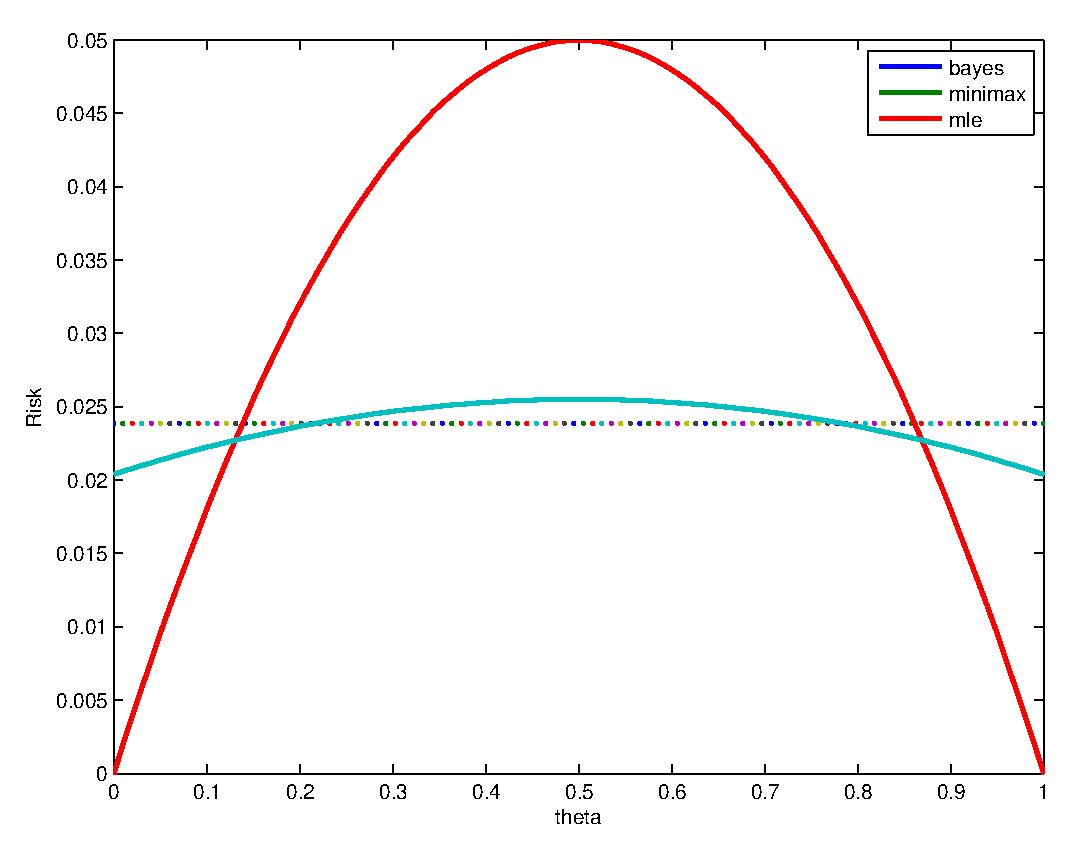
\includegraphics[width=2.2in]{1.eps}
\caption{n=5}
\end{minipage}%
\begin{minipage}[t]{0.3\linewidth}
\centering
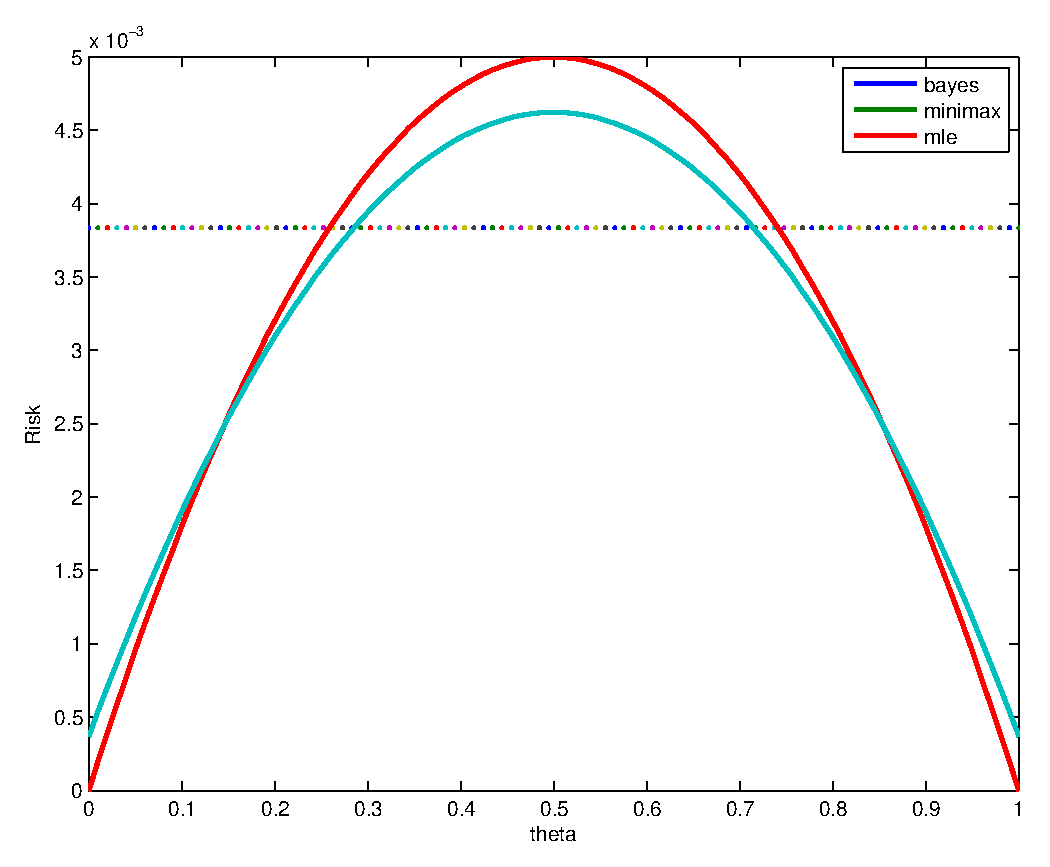
\includegraphics[width=2.2in]{2.eps}
\caption{n=50}
\end{minipage}
\begin{minipage}[t]{0.3\linewidth}
\centering
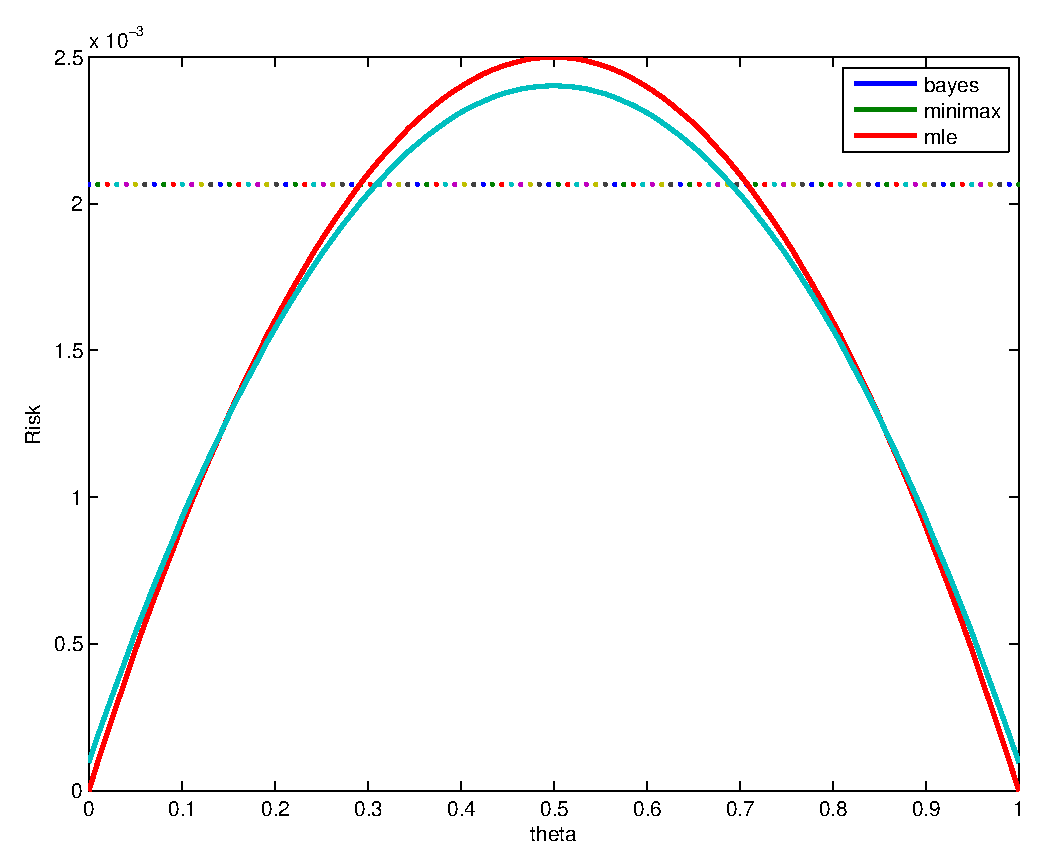
\includegraphics[width=2.2in]{3.eps}
\caption{n=100}
\end{minipage}
\end{figure}
\section*{Programming}
In this problem you will implement Naive Bayes and Logistic Regression, then compare their performance on a
document classification task. The data for this task is taken from the 20 Newsgroups data set, and is available
from the attached zip file. The included README.txt describes the data set and file format.

Our Naive Bayes model will use the bag-of-words assumption. This model assumes that each word in a
document is drawn independently from a multinomial distribution over possible words. (A multinomial
distribution is a generalization of a Bernoulli distribution to multiple values.) Although this model ignores
the ordering of words in a document, it works surprisingly well for a number of tasks. We number the words
in our vocabulary from 1 to $m$, where $m$ is the total number of distinct words in all of the documents.
Documents from class $y$ are drawn from a class-specific multinomial distribution parameterized by $\theta_y$. $\theta_y$ is
a vector, where $\theta_{y,i}$ is the probability of drawing word $i$ and $\sum_{i=1}^m \theta_{y,i}=1$.
Therefore, the class-conditional probability of drawing document x from our Naive Bayes model is
$P(X = x|Y = y) = \prod_{i=1}^m (\theta_{y,i})^{count_i(x)}$, where $count_i(x)$ is the number of times word $i$ appears in $x$.

1. Provide high-level descriptions of the Naive Bayes and Logistic Regression algorithms. Be
sure to describe how to estimate the model parameters and how to classify a new example.\\
\emph{\textbf{SOLUTION}}:\\
\begin{itemize}
\item Naive Bayes model  model
\begin{equation}\nonumber
\begin{aligned}
P(Y=y|X=x)&=\frac{P(X=x|Y=y)P(Y=y)}{P(X=x)}\\
&=\frac{P(Y=y)\prod_{i=1}^m (\theta_{y,i})^{count_i(x)}}{P(X=x)}
\end{aligned}
\end{equation}

\begin{equation}\nonumber
\begin{aligned}
\hat{Y}&=\mathop{\argmax}_{y} P(Y=y|X=x)\\
\hat{Y}&=\mathop{\argmax}_{y} P(Y=y)\prod_{i=1}^m (\theta_{y,i})^{count_i(x)}
\end{aligned}
\end{equation}

\item Logistic Regression model \[P(Y=y|X=x)=\frac{1}{1+e^{-\mathbf{w}^Tx}}, \mathbf{w}=[w_0,w_1,\cdots,w_m]^T\]
for this model, we need to estimate the only parameter $\mathbf{w}$ by maximizing the log-likelihood $l(\mathbf{w})$:
\begin{equation}\nonumber
\begin{aligned}
\hat{\mathbf{w}}&=\mathop{\argmax}_{w} l(\mathbf{w})\\
\hat{\mathbf{w}}&=\mathop{\argmax}_{w} \ln(\prod_j \frac{1}{1+e^{-\mathbf{w}^Tx^j}})
\end{aligned}
\end{equation}
\end{itemize}
we can solve the above equation by gradient descent.

2. Imagine that a certain word is never observed in the training data, but occurs in a test
instance. What will happen when our Naive Bayes classifier predicts the probability of the this test
instance? Explain why this situation is undesirable. How to avoid this problem? Will logistic regression have a similar problem?
Why or why not?\\
\emph{\textbf{SOLUTION}}:\\
Naive Bayes classifier predicts the probability of unobserved instance to be 0. We can avoid this problem using add-one
smoothing when estimating the parameters. It pretend every word occurs at least one time by adding one additional time
for every word.\\
Logistic Regression will not have this problem. For a word $i$ is not observed in the training set, then $w_i*x_i$ will be 0,
which means the model will ignore the unobserved word.

3. Implement Logistic Regression and Naive Bayes. Use add-one smoothing when estimating
the parameters of your Naive Bayes classifier. For logistic regression, we found that a step size around
0.0001 worked well. Train both models on the provided training data and predict the labels of the test
data. Report the training and test error of both models. Submit your code along with your homework.\\
\emph{\textbf{SOLUTION}}:\\
\begin{table}[!htbp]
\centering
\begin{tabular}{|c|c|c|}
\hline
 Algorithm& Training Error & Test Error\\
\hline
Naive Bayes & 0.057 & 0.215 \\
\hline
Logistic Regression & 0.083 & 0.223 \\
\hline
\end{tabular}
\caption{Predictions from the Naive Bayes}
\end{table}
4. Which model performs better on this task? Why do you think this is the case?\\
\emph{\textbf{SOLUTION}}:\\
The performance of Naive Bayes and Logistic Regression are the same. Because we don't have enough training data,
the model may be overfited.

%%%%%%%%%%%%%%%%%%%%%%%%%%%%%%%%%%%%%%%%%%%%%%%%%%%%%%%%%%%%%%%%%%%%
% Reference
%%%%%%%%%%%%%%%%%%%%%%%%%%%%%%%%%%%%%%%%%%%%%%%%%%%%%%%%%%%%%%%%%%%%
%\begin{thebibliography}{1}

%\bibitem{BoydVandenberghe2004}
%S. Boyd and L. Vandenberghe, \emph{Convex Optimization}, Cambridge
%University Press, 2004.

%\end{thebibliography}
\end{document}
